\documentclass[14pt]{beamer}

% Presento style file
\usepackage{config/presento}

% custom command and packages
% custom packages
\usepackage{textpos}
\setlength{\TPHorizModule}{1cm}
\setlength{\TPVertModule}{1cm}

\newcommand\crule[1][black]{\textcolor{#1}{\rule{2cm}{2cm}}}



% Information
\title{Drumtranscription}
\subtitle{Detect drums in polyphonic sound}
\author{Anyere Bendrien \\ Maximilian Wagenbach}
\institute{Audio Content Analysis \\ TU Berlin}
\date{\today}

\begin{document}
% Title page
\begin{frame}[plain]
\maketitle
\end{frame}

\notosansfont

% sections in the presentation
\begin{frame}{Drumtranscription}
 \begin{fullpageitemize}
  \item Detect percussive events in polyphonic sound
  \item Onset and Type (Bassdrum, Hi Hat, Snare, ...)
  
  \item \textbf{Optional:} \\
        Visualization of drum onsets
  \item Tempodetection / Beat Grid [2]
 \end{fullpageitemize}
\end{frame}

\begin{frame}{Non-negative Matrix Factorization}
 \begin{fullpageitemize}
  \item 
  \begin{figure}
   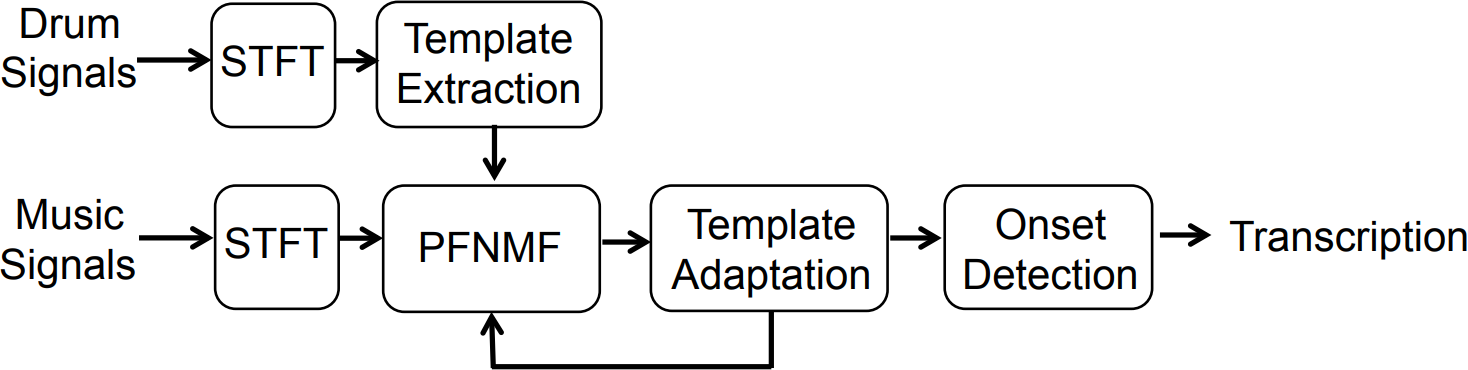
\includegraphics[width=\textwidth]{images/Flowchart.png}
   \caption{Flowchart of the drum transcription system [1]}
  \end{figure}
  \notosansfont
  \item 
 \end{fullpageitemize}
\end{frame}

\begin{frame}
 \frametitle{References}
  {\small [1] Chih-Wei Wu, Alexander Lerch. “Drum Transcription Using Partially Fixed Non-Negative Matrix Factorization with Template Adaptation”, 16th International Society for Music Information Retrieval Conference, 2015}\\
  {\small [2] Daniel Gärtner. “Tempo Detection Of Urban Music Using Tatum Grid Non-Negative Martix Factorizytion”, International Society for Music Information Retrieval, 2013}
\end{frame}

\framecard[colorgreen]{{\color{white}\hugetext{Thanks for listening!}}}

\end{document}